\documentclass{article}
\usepackage[T1]{fontenc}
\usepackage{lmodern}
\usepackage{graphicx}
\usepackage{amsmath,amssymb}
\usepackage[a4paper,margin=2cm]{geometry}
\usepackage[absolute,overlay]{textpos}
\setlength{\TPHorizModule}{1mm}
\setlength{\TPVertModule}{1mm}
\usepackage[indonesian]{babel}
\usepackage{hyperref}
\setlength{\emergencystretch}{2em}
% unit: Halaman 59

\begin{document}

% === Halaman 59 (llm) ===

\vspace{196.02mm}

\textbf{Plaintext input}
\vspace{50mm}
\textbf{Ciphertext}
\vspace{50mm}
\textbf{Plaintext output}
\vspace{80mm}
Sumber: Cryptography in E-Commerce

% deskripsi: Diagram proses enkripsi dan dekripsi simetris yang menunjukkan penggunaan kunci yang sama (shared secret) untuk mengubah plaintext menjadi ciphertext dan kembali menjadi plaintext.
% bbox normalisasi: [0.1500, 0.1900, 0.7600, 0.8500]
\begin{textblock*}{128.10mm}(31.50mm,56.43mm)
\noindent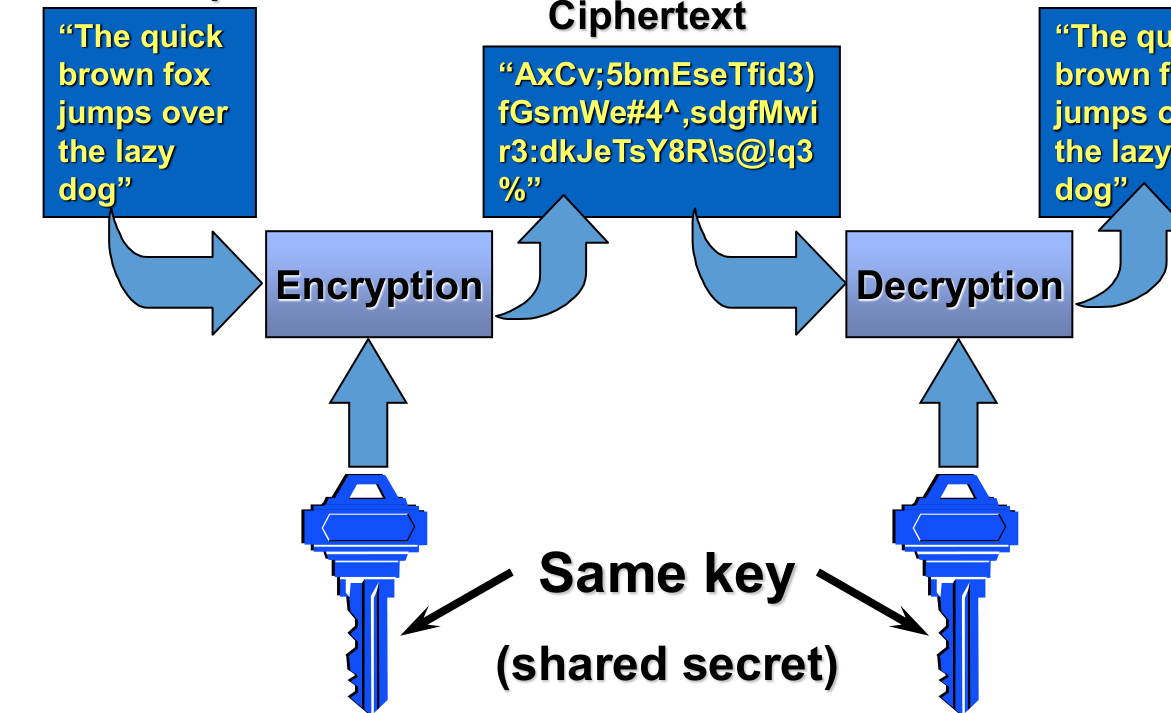
\includegraphics[width=128.10mm,height=196.02mm]{../../images/llm/page_059_img_01.png}%
\end{textblock*}

\end{document}
